% !TEX root =  podc-submission.tex

\section{Reducing Space}
\label{reducing}
\paragraph{Reducing Space Usage}
The \nf{blocks} arrays defined in our algorithm are unbounded. To use $O(n)$ space in each node where $n$ is the total number of operations, instead of unbounded arrays, we could use the memory model of the wait-free vector introduced by Feldman, Valera-Leon and Damian~\cite{7073592}. We can create an array called \nf{arr} of pointers to array segments (see Figure \ref{fig::doublingArray}). When a process wishes to write into location \nf{head} it checks whether \nf{arr[$\lfloor\log $ head$\rfloor$]} points to an array or not. If not, it creates a shared array of size $2^{\lfloor\log \nf{head} \rfloor}$ and tries to \nf{CAS} a pointer to the created array into \nf{arr[$\lfloor\log $ head$\rfloor$]}. Whether the \nf{CAS} is successful or not, \nf{arr[$\lfloor\log $ head$\rfloor$]} points to an array. When a process wishes to access the $i$th element it looks up \nf{arr[$\lfloor\log i\rfloor$][$i-2^{\lfloor\log i\rfloor}$]}, which takes $O(1)$ steps. The CAS Retry Problem does not happen here because if $n$ elements are appended to the array, then only $O(p\times\log n)$ \nf{CAS} steps have happened on the array \nf{arr}. Furthermore, at most $p$ arrays with size $2^{\lfloor\log i\rfloor}$ are allocated by processes while processes try to do the \nf{CAS} on \nf{arr[$i$]}. Jayanti and Shun \cite{DBLP:conf/wdag/JayantiS21} present a way to initialize wait-free arrays in constant steps. The time taken to allocate arrays in an execution containing $n$ operations is $O(\frac{p\log n}{n})$  per operation, which is negligible if $n>>p$. The vector implementation also has a mechanism for doubling \nf{arr} when necessary, but this happens very rarely since increasing \nf{arr} from $s$ to $2s$ increases the capacity of the vector from $2^s$ to $2^{2s}$.
\begin{figure}[hbt]  
  \center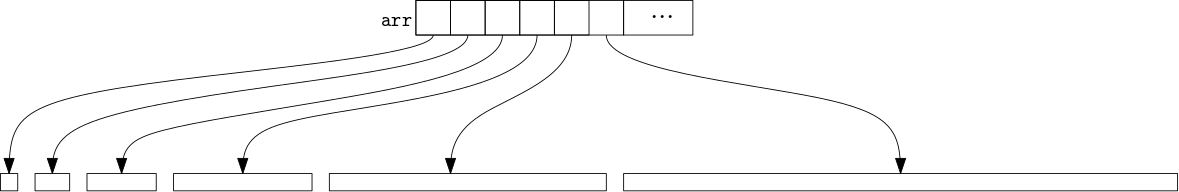
\includegraphics[width=6.5in]{pics/doublingArray.png}
  \caption{Array segments.}
  \label{fig::doublingArray}
\end{figure}

\paragraph{Garbage Collection}
We did not handle garbage collection: \nf{Enqueue} operations  remain in the nodes even after their elements have been dequeued.
We can keep track of the \nf{block}s in the \nf{root} whose operations are all terminated, i.e., all enqueues have been dequeued, and the responses of all dequeues have been computed. We call these blocks \it{finished blocks}. If we help the operations of all processes to compute their responses, then we can say if block $B$ is finished, then all blocks before $B$ are also finished. Knowing the most recent finished block in a node, we can reclaim the memory taken by finished blocks. We cannot use arrays (or vectors) to throw the garbage blocks away. We need a data structure that supports \nf{tryAppend()}, \nf{read(i)}, \nf{write(i)} and \nf{split(i)} operations in $O(\log n)$ time, where \nf{split(i)} removes all the indices less than~\nf{i}. If each process tries to do the garbage collection once every $p^2$ operations on the queue, then the amortized complexity remains the same. We can use a concurrent implementation of a persistent red-black trees for this~\cite{DBLP:conf/afp/Okasaki96}. Bashari and Woelfel ~\cite{DBLP:conf/podc/BashariW21} used persistent red-black trees in a similar way.

Tarjan \cite[Sec.~4.2]{Tar83} described a split algorithm for red-black trees that runs in logarithmic time.
Mention that known lock-free search trees have step complexity that includes a term linear in $p$ \cite{EFHR14,Ko20}.  But we do not need the full functionality:  in particular, we need an operation that tries to insert a node that is allowed to fail if a concurrent insertion occurs for our refresh operation.

\begin{figure}[hbt]  
  \center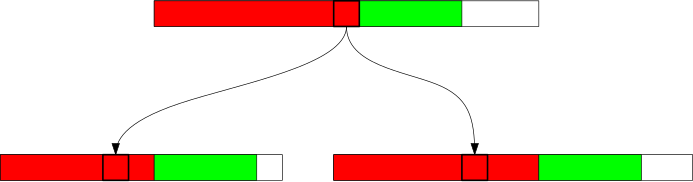
\includegraphics[width=3.5in]{pics/finishedBlocks.png}
  \caption[Blocks that can be safely garbage collected.]{Finished blocks are shown with red color and unfinished blocks are shown with green color. All the subblocks of a finished block are also finished.}
  \label{fig::finishedBlock}
\end{figure}
